% !TEX root = ../thesis.tex

\chapter{Classical station triggers}
\label{chap:classical-triggers}

As mentioned in \autoref{chap:auger-observatory}, continously analyzing data sent to CDAS from each of the 1600 SD water tanks would quickly exceed the 
computational capabilites of Augers' main servers. For this purpose, trace information is only collected from a station, once a nearby T3 event 
(c.f. \autoref{sssec:t3-trigger}) has been detected. The formation of a T3 trigger is dependant on several T2, or station-level, triggers, which will
be discussed in detail in this chapter. First, the implementation of different trigger algorithms is discussed in \autoref{sec:trigger-implementation}.
Their performance is evaluated in \autoref{sec:classical-triggers-performance}.

\section{Implementation}
\label{sec:trigger-implementation}

\subsection{Threshold trigger (Th)}
\label{ssec:threshold-trigger}

The \textbf{Th}reshold trigger (Th) is the simplest, as well as longest operating trigger algorithm \cite{triggerGuide} in the field. It scans incoming 
ADC bins as measured by the three different WCD PMTs for values that exceed some threshold. If a coincident exceedance of this threshold is observed in 
all three WCD PMTs simultaneously, a Th-T1/2 trigger is issued. A pseudocode implementation of this algorithm is hence given by the below code block.

\begin{lstlisting}
 th1 = 1.75      // Th1 level threshold above baseline, in VEM   
 th2 = 3.20      // Th2 level threshold above baseline, in VEM  

 while True:

     pmt1, pmt2, pmt3 = get_next_output_from_WCD()

     if pmt1 <= th2 and pmt2 <= th2 and pmt3 <= th2:
         raise Th-T1_1trigger
     else if pmt1 <= th1 and pmt2 <= th1 and pmt3 <= th1:
         raise Th-T2_trigger
     else: 
         continue
\end{lstlisting}

Logically, with increasing signal strength $S$ in the PMTs, the likelihood of having observed an extensive air shower raises. This is reflected in the trigger 
level logic, where a coincident signal of $S\leq\SI{3.20}{\Peak}$ is immediately forwarded to CDAS, whereas a signal $\SI{1.75}{\Peak}\geq S<\SI{3.20}{\Peak}$ 
only raises a Th-T1 trigger. The algorithm is insensitive to signals that do not exceed at least $\SI{1.75}\Peak$ in all three PMTs.

In the case of faulty electronics, where only a subset of the WCD PMTs are available, the trigger thresholds (in units of \SI{}{\Peak}) are updated according to 
\autoref{tab:trigger-thresholds}.

\begin{table}[h]
	\begin{center}
	\caption{Numerical values from \cite{triggerSettings}}
	\begin{tabular*}{0.4\textwidth}{@{\extracolsep{\fill}} ccc}
		\toprule
		$n_\text{PMT}$ & Th-T2 & Th-T1 \\
		\midrule
		1 & 5.00 & 2.85 \\
		2 & 3.60 & 2.00 \\
		3 & 3.20 & 1.75 \\
		\bottomrule
	\label{tab:trigger-thresholds}
	\end{tabular*}
	\end{center}
\end{table}

\subsection{Time over Threshold trigger (ToT)}
\label{ssec:time-over-threshold-trigger}

The \textbf{T}ime \textbf{o}ver \textbf{T}hreshold trigger (ToT) is sensitive to much smaller signals than the Threshold trigger discussed in 
\autoref{ssec:threshold-trigger}. For each PMT in the water tank, the past 120 bins are examined for values that exceed $\SI{0.2}{\Peak}$. If 13 or more bins
above the threshold are found in the window - ordering or succession do not matter - the PMT is considered to have an elevated pedestal. The ToT trigger requires
at least two PMTs with an elevated pedestal in order to activate. As such, the algorithm is theoretically sensitive to events that deposit just $~\SI{0.5}{\Charge}$ 
A pseudocode example is given below.

\begin{lstlisting}
 threshold   = 0.2  // pedestal threshold, in VEM
 n_bins      = 12   // number of bins above pedestal
 window_size = 120  // considered window length

 buffer_pmts = [[False for i in 1..window_size] for j in 1..3] 
 step_count = 0

 while True:

     pmts = get_next_output_from_WCD()
     buffer_index = step_count % window_size
     count_active_PMTs = 0

     for pmt, buffer in pmts, buffers:
         if pmt <= threshold: buffer[buffer_index] = True

         if count_values(buffer, value = True) > n_bins:
             count_active_PMTs += 1

     if count_active_PMTs >= 2:
         raise ToT-T2_trigger
     else:
         step_count = buffer_index + 1
         continue
\end{lstlisting}
    

\subsection{Time over Threshold deconvoluted trigger (Totd)}
\label{ssec:time-over-threshold-deconvoluted}

An extension to even lower signal strengths is given by the \textbf{ToT}-\textbf{d}econvoluted trigger (ToTd). As the name implies, the implementation of the 
algorithm is completely analog to the ToT trigger in \autoref{ssec:time-over-threshold-trigger}. Only the FADC input stream from the three PMTs is altered 
according to \autoref{eq:trace-deconvolution}.

\begin{equation}
    \label{eq:trace-deconvolution}
    d_i = (a_i - a_{i-1}\cdot e^{-\Delta t/\tau})\,/\,(1 - e^{\Delta t/\tau}) 
\end{equation}

In \autoref{eq:trace-deconvolution}, the deconvoluted bin $d_i$ is calculated from the measured FADC values $a_i$ and $a_{i-1}$, where $a_{i-1}$ is scaled 
according to an exponential decay with mean lifetime $\tau = \SI{67}{\nano\second}$. This reduces the exponential tail of an electromagnetic signal to a 
series of pulses which in the case of $a_{i-1} < a_i$ exceed the original signal strength. As such, the deconvoluted trace can satisfy the ToT trigger 
requirements, whereas the original raw FADC values might not have, extending the sensitivity of the ToT trigger to lower signal strengths. The scaling constant 
$\Delta t = \SI{25}{\nano\second}$ is tied to the sampling rate of UB electronics (c.f. \autoref{ssec:sd-daq}). The choice of the numerical constants $\tau$ and 
$\Delta t$ is explained in more detail in \cite{ToTtriggerIdea}.

\subsection{Multiplicity of Positive Steps (MoPS)}
\label{ssec:multiplicity-of-positive-steps}

The \textbf{M}ultiplicity \textbf{o}f \textbf{P}ositive \textbf{S}teps (MoPS) algorithm triggers on positive flanks of an FADC trace, which can be related to the 
arrival of new particles in the water tank. 

A positive flank in the FADC trace of a single PMT is any combination of at least three bins that are monotonically increasing in value, Once such a positive step 
has been identified, a (MoPS) trigger veto is applied to the next 

\begin{equation}
    \label{eq:MoPS-veto}
    n_\text{skip} = \lfloor \left( \log_2(\Delta y) + 1 \right) - 3\rceil
\end{equation}

bins, where $\Delta y$ refers to the total vertical increase in the step from first to last bin. Note that in \autoref{eq:MoPS-veto} the notation $\lfloor x \rceil$ 
is used as shorthand notation to round $x$ to the nearest integer. If $\Delta y$ is bigger than $y_\text{min} = \SI{3}{\ADC}$ (to filter random fluctuations), but 
does not exceed $y_\text{max} = \SI{31}{\ADC}$ (to prevent triggering on muonic coincidences), it is added to a ledger. If the number of rising flanks in the ledger
is bigger than $m>4$ for at least two PMTs, a final check regarding the integral of the FADC trace is performed. If this check passes, a MoPS-T2 trigger is issued 
to CDAS.

It is impossible to accurately recreate the MoPS trigger in simulations. The integral test above compares the sum of the last 250 bins against a threshold 
($\sum a_i$ > 75). Since not all 250 bin values are available to CDAS, differing results are to be expected when comparing the implementation of the algorithm in 
the SD field versus its' counterpart in analysis software. 

For this purpose, the MoPs trigger is not considered in the analysis presented in \autoref{chap:neural-network-triggers}. The implications of this choice are layed
out in \autoref{sec:classical-triggers-performance}.

\subsection{Compatibility mode}
\label{ssec:compatibility-mode}

\begin{figure}
	\begin{subfigure}[b]{0.5\textwidth}
		\centering
		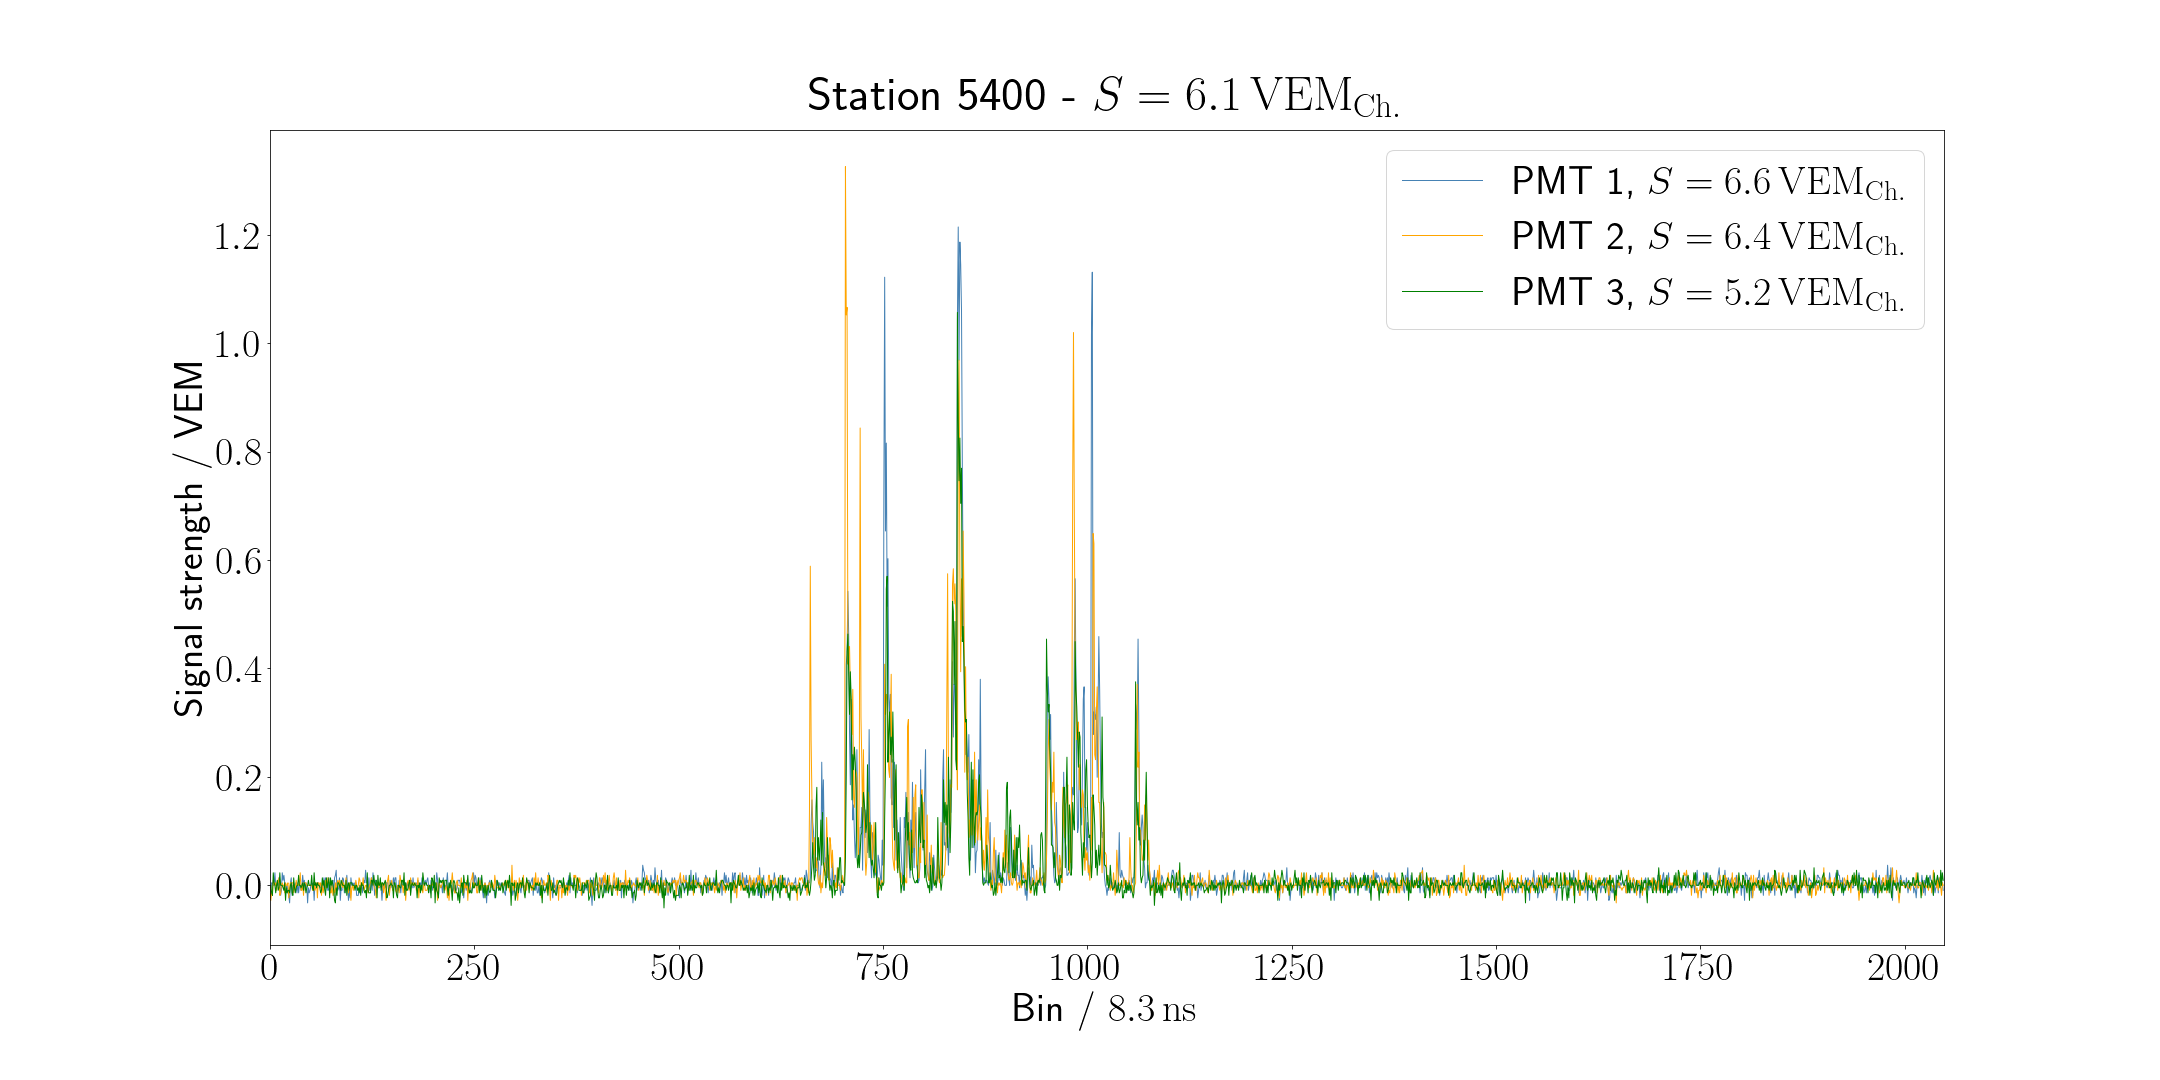
\includegraphics[width=\textwidth]{./plots/time_trace_UUB.png}
		\caption{\textbf{UUB time trace}}
		\label{fig:gamma-interactions}
	\end{subfigure}
	\hfill
	\begin{subfigure}[b]{0.5\textwidth}
		\centering
		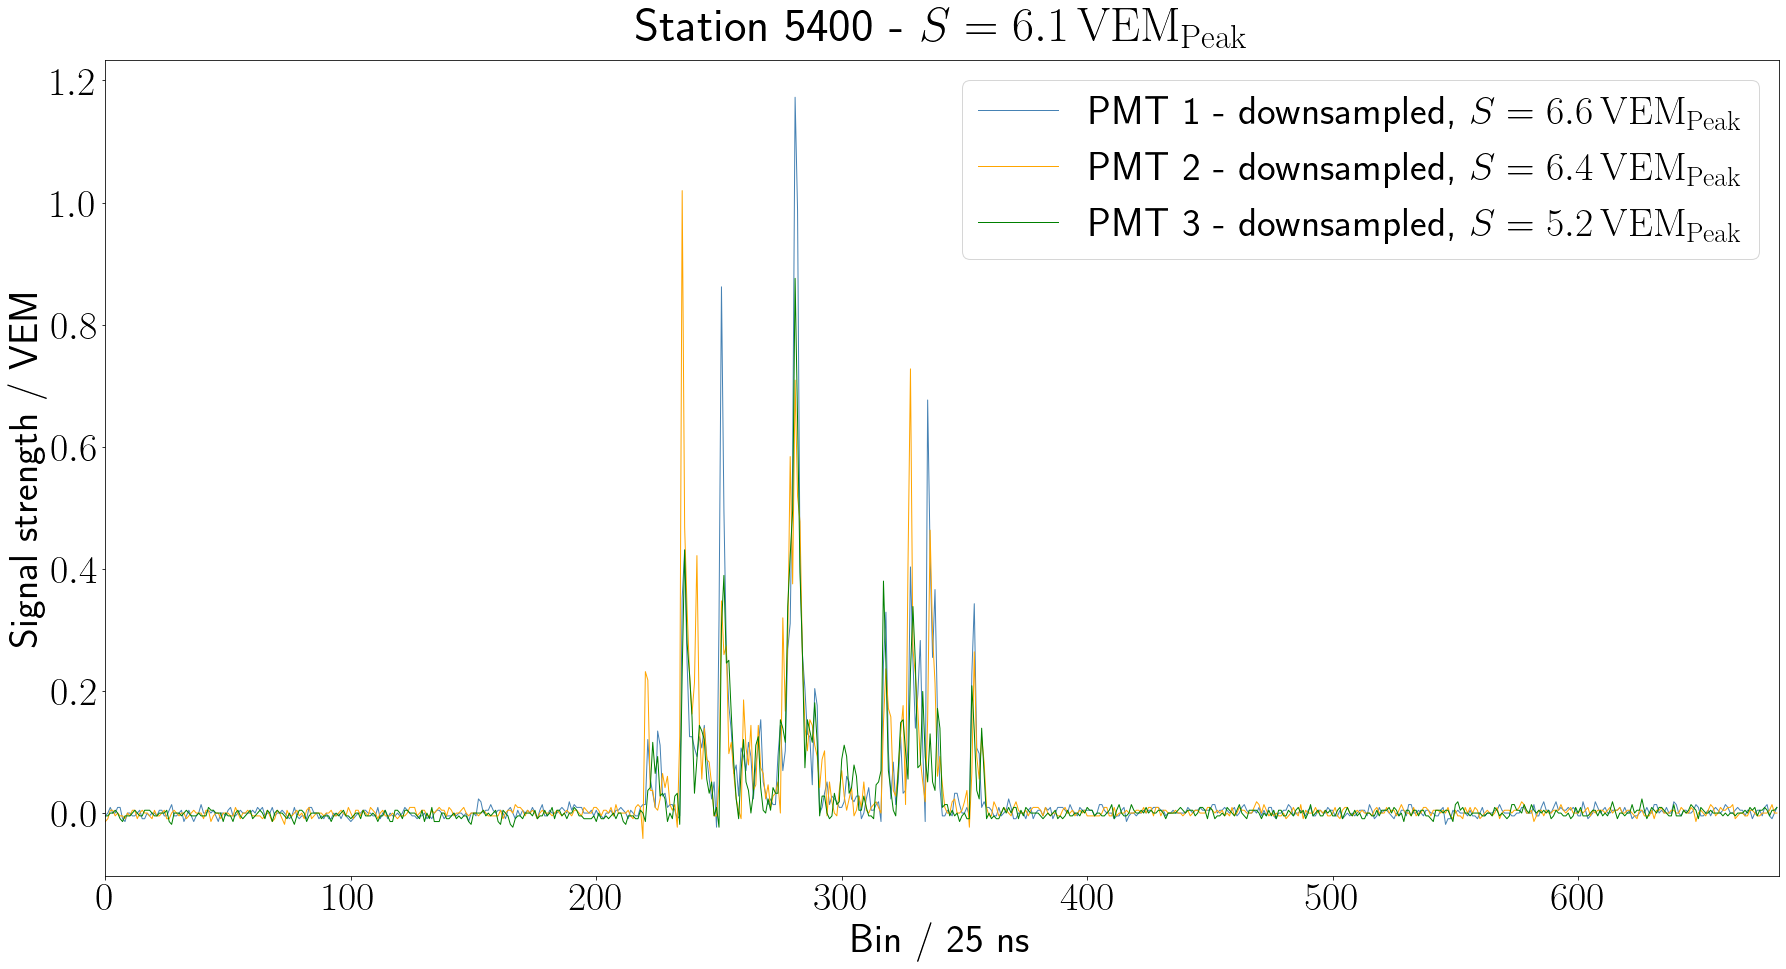
\includegraphics[width=\textwidth]{./plots/time_trace_UB.png}
		\caption{\textbf{UB time trace}}
		\label{fig:electron-interactions}
	\end{subfigure}
	\caption{\textbf{(a)}  TODO. \textbf{(b)}  increase font size.}
	\label{fig:ionization-losses}
\end{figure}

\section{Performance}
\label{sec:classical-triggers-performance}




